% !TeX root = ../thuthesis-example.tex

\begin{translation}
\label{cha:translation}

\title{投影动力学:融合约束投影以实现快速模拟}
\maketitle

\begin{figure}
  \centering
  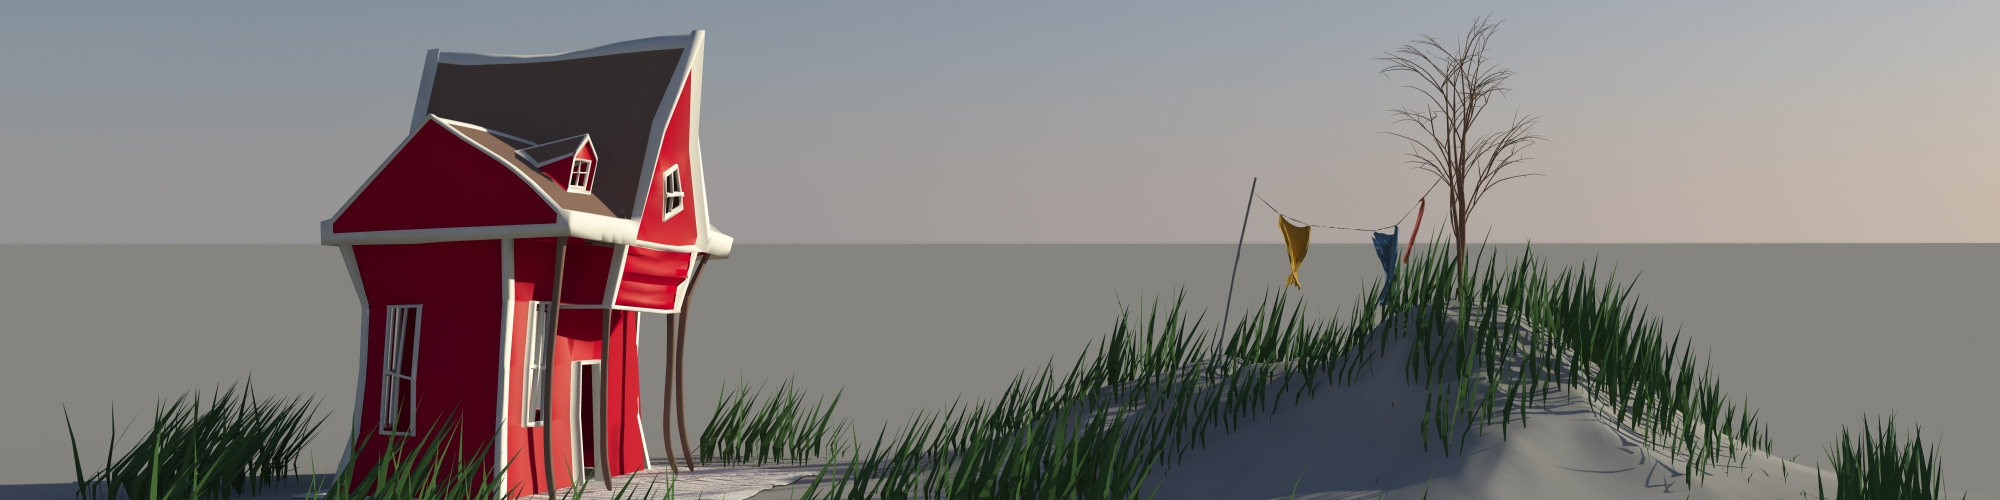
\includegraphics[width = \linewidth]{translation/1.png}
  \caption{
    我们提出了一种新的“基于投影”的隐式Euler积分器,可在单一物理仿真框架中支持多种几何约束。在本示例中,包括建筑物、草地、树木和衣服在内的所有元素(\SI{49}{k}DoFs,\SI{43}{k}约束)都是在\SI{3.1}{\milli\second/iteration}的时间内进行模拟的,每帧迭代10次(另见附带视频)。
  }
  \label{fig:translation-1}
\end{figure}

\begin{abstract}
  我们提出了一种物理系统隐式时间积分的新方法。我们的方法在节点有限元方法和基于位置的动力学之间架起了一座桥梁,从而产生了一种简单、高效、鲁棒而又精确的求解器,支持多种不同类型的约束条件。我们提出了专门设计的势能,可以使用交替优化方法高效求解。受连续介质力学的启发,我们推导出一套基于连续介质的势能,可以有效地集成到我们的求解器中。我们在许多不同的应用中展示了我们方法的通用性和鲁棒性,包括固体、布料和壳体的模拟,以及基于示例的模拟。与牛顿求解器和基于位置的动力学求解器的比较凸显了我们的方法的优势。
\end{abstract}

% \tableofcontents

\section{引言}

基于物理的可变形材料模拟已成为计算机图形学许多领域不可或缺的工具。虚拟世界,以及最近的角色动画,都融入了复杂的模拟以极大地增强视觉体验,例如,通过模拟肌肉、脂肪、头发、衣物或植被。这些模型通常基于连续介质力学公式的有限元离散化,允许高度\emph{精确}地模拟复杂的非线性材料。

除了真实性和准确性,计算机图形学应用中还有许多其他重要的标准。\emph{通用性}是指模拟广泛行为能力的能力,如不同类型的几何体(固体、壳体、杆件)、不同的材料属性,甚至是对经典基于物理的模拟的可控艺术扩展。\emph{鲁棒性}指的是适当处理困难状态的能力,包括大变形、退化几何形状和大时间步长。鲁棒性在实时应用中尤其重要,在这些应用中没有“第二次机会”重新运行模拟,例如在电脑游戏或医学培训模拟器中。求解器的\emph{简单性}对其相关实际应用往往很重要——基于简单、易于理解的概念以及由此产生的轻量级代码库——简化了模拟器的维护,并使其能够适应特定的应用需求。\emph{性能}是实时应用的关键使能标准。然而,在离线模拟中,性能同样重要,应尽量减少测试新场景和模拟参数的周转时间。

当前的连续介质力学方法在计算机图形学应用中的某些方面往往存在不利的权衡,这催生了替代方法的发展,例如基于位置的动力学(PBD)。由于其通用性、简单性、鲁棒性和效率,PBD现在已经在包括PhysX、Havok Cloth、Maya nCloth和Bullet在内的一系列高阶产品中实现。虽然主要用于实时应用,但PBD也经常用于离线模拟。然而,PBD的理想特性是以有限的准确性为代价的,因为PBD并不是从连续体力学原理中严格推导出来的。

我们提出了一种新的隐式积分求解器,它弥合了连续体力学和PBD之间的差距。关键思想是引入具有特定结构的势能。更准确地说,我们的势能由一个凸二次距离度量组成,该度量来自一个\emph{约束}。约束是表达元素期望状态的一般非线性函数,例如,四面体的体积必须保持在给定的范围内。距离度量量化了在给定变形状态中各个约束被违反的程度。虽然我们的求解器可以处理任意的几何约束,但我们提出了一组特定的约束,这些约束源自连续应变能。这些基于连续体的约束非常实用,因为它们大大简化了参数调整,特别是在处理不同分辨率和非均匀细分的网格时。

我们基于约束的势能的主要优势在于,它们的结构使得能够进行高效的局部/全局优化(块坐标下降)。具体来说,局部优化步骤将每个元素投影到约束流形上,即,为每个元素解决一个小的非线性问题。全局优化步骤结合了个体投影的结果,找到所有个体约束之间的折中方案,同时也考虑了全局效应,如惯性和外力。

局部/全局方法使我们能够制定一个隐式积分求解器,它保证在每次迭代中弱减少能量,而不需要任何特定的预防措施。这与经典的牛顿方法相比,后者需要线性搜索策略和防范奇异或不定Hessian矩阵以保证鲁棒性。此外,对于固定的约束集,我们可以预先分解全局步骤的线性系统,这大大减少了计算时间。局部步骤由小的独立优化问题组成,这些问题都可以并行执行。

据我们所知,我们的方法是第一个将局部/全局优化应用于模拟一般动力系统的方法。我们证明了这种解决方案提供了一种鲁棒且高效的隐式积分方法,通常显著优于经典的牛顿方法。PBD与我们的求解器之间的联系揭示了PBD如何与基于有限元方法和牛顿力学的传统方法相关的新见解。

\section{相关工作}

自从Terzopulous及其同事在1987年的开创性工作以来[1987],源自连续介质力学的模型在基于物理的动画中扮演了重要角色。基本原理是,弹性物体对变形的抵抗力是通过弹性势能量化的——一个标量函数,其变分导数导出弹性力[Sifakis and Barbic 2012]。不幸的是,即使是基本的材料模型,弹性力通常也是非线性的,这使得运动方程的时间积分变得复杂。

计算机图形学中使用的最简单的时间积分方案是显式的,对大时间步长非常脆弱[Press et al. 2007]。隐式Euler方法显著提高了鲁棒性[Baraff and Witkin 1998],但代价是在每一步都要解一个非线性方程组。正如[Martin et al. 2011]所示,这可以等效地表述为一个直接作用于弹性势能而非力的非凸优化问题。隐式积分的一个主要缺点是人为的数值阻尼。这启发了辛积分器[Hairer et al. 2002; Kharevych et al. 2006]和混合隐式-显式方法(IMEX)[Bridson et al. 2003; Stern and Grinspun 2009]的发展,它们具有更好的能量守恒特性。另一种方法是\emph{energy budgeting}[Su et al. 2013],它显式地强制能量守恒。然而,隐式Euler积分继续是物理动画应用中的一个受欢迎的选择,其中鲁棒性是一个重要标准,数值阻尼不是主要关注点。我们的求解器是从隐式Euler积分的变分形式[Martin et al. 2011]衍生出来的,因为它为我们的框架中的时间积分提供了一种直观的思考方式——仅仅通过向系统添加另一个约束。这进一步允许我们在PBD和隐式Euler积分方案之间建立联系,并导出一种鲁棒且高效的方法,该方法在大时间步长下稳定。

不管隐式积分的具体形式和表述如何,牛顿法仍然是解决非线性方程组的主要方法。然而,其鲁棒实现需要采取预防措施,如保守的线搜索程序和对不定Hessian的防范[Boyd and Vandenberghe 2004]。从性能的角度来看,牛顿法的一个严重缺点是Hessian矩阵和梯度在每次迭代时都会变化。因此,拟牛顿法采用近似Hessian,用次优的下降方向换来更快的线性系统求解(因此收敛速度更慢),正如[Desbrun et al. 1999; Hahn et al. 2012]所示。在共旋弹性的背景下探索的一种类似策略是使用精心调度的稀疏Cholesky分解更新[Hecht et al. 2012]。最近,Liu及其同事[2013]提出了一种高效隐式时间积分质点-弹簧系统的方法,通过引入辅助变量来实现局部/全局优化的交替。这种方法,也被称为块坐标下降法,之前已在几何处理中取得了巨大成功[Sorkine and Alexa 2007; Bouaziz et al. 2012]。我们的方法也采用了局部/全局交替,但与[Liu et al. 2013]不同的是,后者仅限于质量-弹簧系统,并且\emph{只}假设线性弹簧(胡克定律),我们展示了如何通过将投影概念推广到约束集上来模拟\emph{一般的}节点动力系统。

我们基于约束的公式与基于约束投影的最新非传统方法有些相似。约束投影的概念是Nucleus系统[Stam 2009]和基于位置的动力学[Müller et al. 2007; Bender et al. 2013]的核心。与我们的解决方案不同,这些方法并没有以全局方式处理约束,而是以(非线性的)Gauss-Seidel类似的方式迭代地投影到它们上[Müller et al. 2007]。虽然得到的算法非常容易实现,但这种方法有一些缺点:Gauss-Seidel优化的收敛速度不是很快,材料刚度取决于迭代次数,结果依赖于遍历顺序。相比之下,我们的方法使用约束来制定弹性势能,这些势能与牛顿运动定律所规定的惯性项严格结合。我们的求解器首先分别计算所有约束投影,然后找到它们之间的最佳折衷,这使得解决方案不依赖于约束的顺序。为了获得更快的收敛速度,约束是用微分坐标表示的,这通常在仅几次迭代后就能得到令人满意的结果。此外,与基于位置的动力学不同,我们的求解器收敛到一个真正的隐式Euler解,带有我们的弹性能量,而基于位置的动力学收敛到完全无弹性的行为。

另一个与我们的方法密切相关的概念是形状匹配[Müller et al. 2005; Rivers and James 2007],与我们的方法不同的是,约束投影被用来直接构建弹性力而不是势能来模拟可变形物体。约束投影也被用于\emph{应变限制}[Provot 1995; Goldenthal et al. 2007; Thomaszewski et al. 2009; Wang et al. 2010; Narain et al. 2012],不是作为一种独立的模拟技术,而是作为一种改善标准时间积分方法处理刚性系统的方式。在我们的方法中,我们也可以进行应变限制,但它直接包含在隐式求解器中。

\section{连续介质力学视角}

在本节中,我们将介绍我们方法的基础——我们势能的特殊结构。我们从有限元素法离散的弹性模型的隐式时间积分开始。

\subsection{隐式Euler求解器}

让我们简要回顾一下隐式Euler积分的变分形式[Martin et al. 2011]。我们假设一个由$m$个顶点组成的网格,顶点位置为$\vb{q} \in \mathbb{R}^{m \times 3}$,速度为$\vb{v} \in \mathbb{R}^{m \times 3}$。系统根据牛顿运动定律在一系列离散的时间点$t_1, t_2, \dots$中随时间演化。在时间$t_n$,系统可由$\{\vb{q}_n, \vb{v}_n\}$确定。外力之和为$\vb{f}_{\text{ext}}$,内力之和为$\vb{f}_{\text{int}}$。我们考虑位置依赖的内力,即$\vb{f}_{\text{int}}(\vb{q}) = - \sum_i \grad{W_i(\vb{q})}$,其中$W_i(\vb{q})$是一个标量势能函数。隐式Euler时间积分导出以下更新规则:
\begin{gather}
  \vb{q}_{n + 1} = \vb{q}_n + h \vb{v}_{n + 1} \label{eq:translation-1} \\
  \vb{v}_{n + 1} = \vb{v}_n + h \vb{M}^{-1} (\vb{f}_{\text{int}}(\vb{q}_{n + 1}) + \vb{f}_{\text{ext}}) \label{eq:translation-2}
\end{gather}
其中$\vb{M}$是质量矩阵,$h$代表时间步长。注意,$\vb{f}_{\text{ext}}$和$\vb{M}$在任何给定的时间步长中都是保持不变的。使用这些公式,我们可以推导出
\begin{equation}
  \vb{M} (\vb{q}_{n + 1} - \vb{q}_n - h \vb{v}_n) = h^2 (\vb{f}_{\text{int}}(\vb{q}_{n + 1}) + \vb{f}_{\text{ext}})
  \label{eq:translation-3}
\end{equation}
这个系统可以转换为一个优化问题
\begin{equation}
  \min_{\vb{q}_{n + 1}} \frac{1}{2 h^2} \norm{\vb{M}^{\frac{1}{2}} (\vb{q}_{n + 1} - \vb{s}_n)}_F^2 + \sum_i W_i(\vb{q}_{n + 1})
  \label{eq:translation-4}
\end{equation}
其中$\vb{s}_n = \vb{q}_n + h \vb{v}_n + h^2 \vb{M}^{-1} \vb{f}_{\text{ext}}$,$\norm{\cdot}_F$表示Frobenius范数。直观上,这个最小化问题也即\emph{动量势能}
\begin{equation}
  \frac{1}{2 h^2} \norm{\vb{M}^{\frac{1}{2}} (\vb{q}_{n + 1} - \vb{s}_n)}_F^2
  \label{eq:translation-5}
\end{equation}
这表明解应该遵循其动量(加上外力),以及要求解最小化弹性形变的弹性势能之间的折中。相应的权重项,即$\vb{M}$中的质量分布、时间步长$h$和材料刚度$W$,决定了这种平衡中哪个势能更重要。此外,根据Noether定理,当弹性势能对刚体运动是不变的时,线性和角动量总是守恒的。

公式\eqref{eq:translation-4}的最小化通常使用精心实现的牛顿法来执行[Martin et al. 2011]。然而,这是相当昂贵的,因为在每次迭代中都需要解一个不同的线性系统,因为Hessian从一次迭代到下一次迭代是变化的。为了简化表示,我们将在下文中省略$\vb{q}_{n + 1}$的下标,只使用 $\vb{q}$。

\subsection{非线性弹性力学}

我们分析了基于有限元方法(FEM)的非线性弹性能量的经典形式,以揭示我们如何限制公式\eqref{eq:translation-4}中的弹性势能,以便推导出我们的新型求解器。

\paragraph{非线性弹性势能。}

在非线性连续介质力学中,从静止状态开始的变形是使用离散的元素应变$\vb{E}(\vb{q})$来衡量的,例如,二次Green应变[Irving et al. 2004]。实践中使用的许多弹性势均使用(通常是非线性的)材料模型$\Psi(\cdot)$将其公式化为应变的函数,从而得到弹性势$W(\vb{q}) = \Psi(\vb{E}(\vb{q}))$。从几何角度来看,我们可以观察到$\vb{E}(\vb{q}) = \vb{0}$定义了所有可能未变形状态的约束流形,而$\Psi(\vb{E}(\vb{q}))$度量变形状态与该流形的距离(图~\ref{fig:translation-2}中的等值线)。我们的关键观察是这两个概念可以解耦;距离度量不必是一个复杂的非线性函数,因为非线性已经包含于约束流形。

\begin{figure}
  \centering
  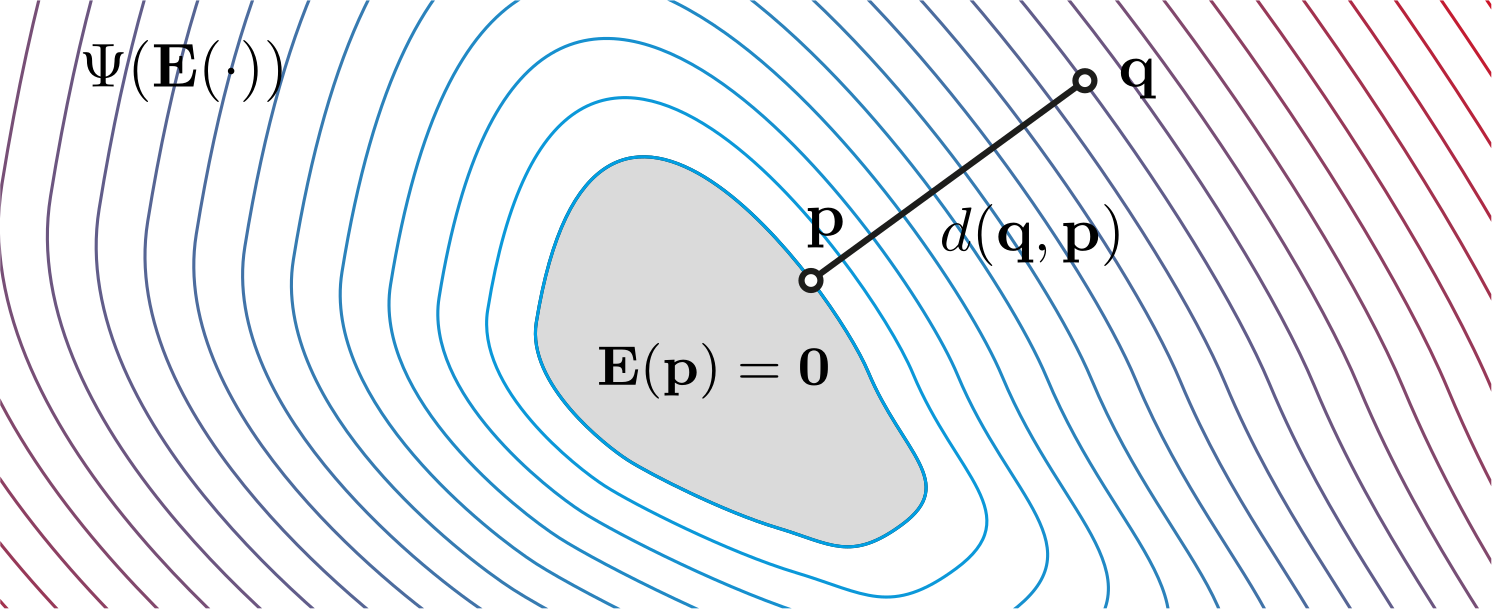
\includegraphics[width = 0.5 \linewidth]{translation/2.png}
  \caption{
    函数$\Psi(\vb{E}(\cdot))$既定义了约束流形$\vb{E}(\cdot) = \vb{0}$作为其零水平集,也定义了由其等值线给出的弹性势能。通过在流形中引入一个投影变量$\vb{p}$,我们可以将流形定义与弹性势能解耦,后者被建模为距离函数$d(\vb{q}, \vb{p}$)。
  }
  \label{fig:translation-2}
\end{figure}

\paragraph{解耦距离度量和约束流形。}

我们引入了使用辅助变量$\vb{p}$的势能函数$W$,定义为
\begin{equation}
  W(\vb{q}, \vb{p}) = d(\vb{q}, \vb{p}) + \delta_{\vb{E}}(\vb{p})
  \label{eq:translation-6}
\end{equation}
这里,$\delta_{\vb{E}}(p)$是一个指示函数,如果$\vb{E}(\vb{p}) = 0$则为零,否则为$+\infty$,并且规定了$\vb{p}$应该位于约束流形上。然后函数$d(\vb{q}, \vb{p})$度量$\vb{q}$和$\vb{p}$之间的距离。关于$\vb{p}$最小化公式\eqref{eq:translation-6}相当于将$\vb{q}$投影到约束流形上,如图~\ref{fig:translation-2}所示。因此,可以定义一个类似于$\Psi(\vb{E}(\vb{q}))$的弹性势能为$W(\vb{q}) = \min_{\vb{p}} W(\vb{q}, \vb{p})$。

\paragraph{二次距离度量。}

考虑到这种解耦,我们可以构建一个求解器,它交替进行距离最小化和投影。这种方法的一个重要优势是距离度量可以自由选择。\emph{约束的非线性}(也称为几何非线性)已经通过对约束集的投影得到处理,因此距离度量可以保持简单,以效率和鲁棒性为代价,而不考虑一般\emph{材料的非线性}。具体来说,我们基于距离矩阵导出以下势能:
\begin{equation}
  W(\vb{q}, \vb{p} = \frac{w}{2} \norm{\vb{A} \vb{q} - \vb{B} \vb{p}}_F^2 + \delta_{\vb{C}(\vb{p})})
  \label{eq:translation-7}
\end{equation}
其中$\vb{A}$和$\vb{B}$是常数矩阵,$w$是非负权重。因此,到约束集的距离通过$\vb{q}$和$\vb{p}$的\emph{二次}函数来建模,这使我们能够使用一个高效的求解器。此外,我们不限于使用Green应变,而可以使用任何约束定义$\vb{C}(\vb{q}) = \vb{0}$来表示所需的状态[Baraff and Witkin 1998],例如,描述三角形之间期望的弯曲角度,四面体的目标体积,或后文所讨论的边界条件。

\subsection{投影隐式Euler求解器}

使用简化的势能,如公式\eqref{eq:translation-7}所示,我们可以将公式\eqref{eq:translation-4}中定义的隐式积分重构为关于$\vb{q}$和辅助变量$\vb{p}_i$最小化
\begin{equation}
  \frac{1}{2 h^2} \norm{\vb{M}^{\frac{1}{2}} (\vb{q} - \vb{s}_n)}_F^2 + \sum_i \frac{w_i}{2} \norm{\vb{A}_i \vb{S}_i \vb{q} - \vb{B}_i \vb{p}_i}_F^2 + \delta_{\vb{C}_i}(\vb{p}_i)
  \label{eq:translation-8}
\end{equation}
其中$\vb{S}_i$是一个恒定的选择矩阵,用于选择参与第$i$个约束的顶点。我们使用局部/全局交替最小化技术来最小化公式\eqref{eq:translation-8}。

\paragraph{局部求解。}

首先,我们在保持位置固定的情况下,对辅助变量进行公式\eqref{eq:translation-8}的最小化。由于每个约束都有自己的一组辅助变量$\vb{p}_i$,所以可以独立地对每个约束进行最小化,即
\begin{equation}
  \min_{\vb{p}_i} \frac{w_i}{2} \norm{\vb{A}_i \vb{S}_i \vb{q} - \vb{B}_i \vb{p}_i}_F^2 + \delta_{\vb{C}_i}(\vb{p}_i)
  \label{eq:translation-9}
\end{equation}
这允许局部步骤的大规模并行化。我们将在第~\ref{sec:translation-continuum-based-constraints}节讨论具体的约束类型。

\paragraph{全局求解。}

其次,我们在保持辅助变量固定的情况下,对位置进行公式\eqref{eq:translation-8}的最小化。由于未知数$\vb{q}$在公式\eqref{eq:translation-8}中是二次的,我们可以通过单次线性求解来最小化它。令临界点处梯度消失,导出线性系统
\begin{equation}
  \pqty{\frac{\vb{M}}{h^2} + \sum_i w_i \vb{S}_i^T \vb{A}_i^T \vb{A}_i \vb{S}_i} \vb{q} = \frac{\vb{M}}{h^2} \vb{s}_n + \sum_i w_i \vb{S}_i^T \vb{A}_i^T \vb{B}_i \vb{p}_i
  \label{eq:translation-10}
\end{equation}
只要约束不变,系统矩阵就是常数,因此可以在初始化时预分解,从而实现非常高效的全局求解。右侧需要在每次迭代后更新投影变量后重新计算。请注意,目标函数是有下界的,而且局部和全局步骤都保证减小它,即使对于非凸集也是如此。因此,优化会收敛,使得不需要额外的安全措施。

\paragraph{算法。}

我们在算法~\ref{alg:translation-1}中总结了我们的优化程序。在第~\ref{alg:translation-1L2}行,我们使用估计动量$\vb{s}_n$来初始化。我们观察到,当只使用少量求解器迭代时,这是有利的,因为它导致的系统阻尼比使用上一个时间步的解作为起点时要小。在求解了多次局部/全局迭代后,速度在第~\ref{alg:translation-1L9}行更新。

\begin{algorithm}
  \caption{投影隐式Euler求解器}
  \label{alg:translation-1}
  \small
  \begin{algorithmic}[1]
    \STATE $\vb{s}_n = \vb{q}_n + h \vb{v}_n + h^2 \vb{M}^{-1} \vb{f}_{\text{ext}}$
    \STATE $\vb{q}_{n + 1} = \vb{s}_n$ \label{alg:translation-1L2}
    \FOR{$iter = 0$ \TO solverIteration}
    \FORALL{constraints $i$}
    \STATE $\vb{p}_i = ProjectOnConstraintSet(\vb{C}_i, \vb{q}_{n + 1})$ \label{alg:translation-1L5}
    \ENDFOR
    \STATE $\vb{q}_{n + 1} = SolveLinearSystem(\vb{s}_n, \vb{p}_1, \vb{p}_2, \vb{p}_3, \dots)$ \label{alg:translation-1L7}
    \ENDFOR
    \STATE $\vb{v}_{n + 1} = (\vb{q_{n + 1} - \vb{q}_n}) / h$ \label{alg:translation-1L9}
  \end{algorithmic}
\end{algorithm}

\paragraph{$\vb{A}$和$\vb{B}$的选取。}

如果我们选取$\vb{A}_i = \vb{B}_i = \vb{I}$,公式\eqref{eq:translation-7}度量的是从$\vb{S}_i \vb{q}$到约束集上最近点的欧式平方距离。由于矩阵是对角的,全局求解的Hessian最终也是对角的,因此可以求解一个简单的线性系统。

如果我们利用内部物理约束是平移不变的事实(即,对约束中涉及的所有点应用共同的平移不会改变约束的值),那么收敛速度可以大大提高。在这种情况下,我们可以选择$\vb{A}_i = \vb{B}_i$作为微分坐标矩阵(它们的零空间中有全局平移)。可以使用各种这样的矩阵,例如可以减去平均值[Bouaziz et al. 2012],或者简单地减去约束中涉及的一个顶点[Liu et al. 2013]。请注意,$\vb{A}_i$ 和 $\vb{B}_i$的选择只影响数值求解过程,并不影响动量守恒。

使用这样的微分坐标大大提高了结果局部/全局求解器的收敛速度[Bouaziz et al. 2012]。然而,如果不采取进一步的预防措施,所得到的行为将依赖于分割和分辨率。我们在第~\ref{sec:translation-continuum-based-constraints}节展示,在某些情况下,$\vb{A}_i$和$\vb{B}_i$矩阵可以从连续体公式中导出,以避免这些缺点。

\section{基于位置的动力学视角}
\label{sec:translation-position-based-dynamics-view}[Liu et al. 2013]揭示了一般变分隐式Euler方法与基于位置的动力学(PBD)之间的相似性,在本节中,我们不仅推导出隐式Euler方法与PBD之间的确切关系,而且还推导出局部/全局公式与PBD之间的关系,适用于一般约束。这一分析突出了PBD与我们的求解器之间的紧密联系,但也指出了根本的差异,这些差异解释了我们的方法获得更高精度结果的原因。

\subsection{Gauss-Seidel求解器}
\label{sec:translation-gauss-seidel-solver}

经典的PBD求解器[Müller et al. 2007]执行三个步骤。在第一步中,通过显式Euler步骤初始化位置,忽略内部力。在第二步中,通过连续对每个约束集进行投影来更新位置,同时考虑质量加权。在最后一步中,速度被更新为$\vb{v}_{n + 1} = (\vb{q}_{n + 1} - \vb{q}_n) / h$。

我们可以证明,PBD的约束求解策略实际上实现了对能量的Gauss-Seidel类型最小化
\begin{equation}
  \frac{1}{2} \sum_i \norm{\vb{M}_i^{\frac{1}{2}} (\vb{S}_i \vb{q} - \vb{p}_i)}_F^2 + \delta_{C_i}(\vb{p}_i)
  \label{eq:translation-11}
\end{equation}
这里使用了一个仅涉及约束点的集中质量矩阵$\vb{M}_i$。Gauss-Seidel方法通过顺序优化每个求和项来最小化这个能量,即,最小化形如$\frac{1}{2} \norm{\vb{M}^{\frac{1}{2}} \Delta\vb{q}}_F^2 + \delta_C(\vb{q} + \Delta\vb{q})$的势能,我们引入修正$\Delta\vb{q} = \vb{p} - \vb{q}$来简化推导。使用拉格朗日乘数对线性化约束$C(\vb{q}) + \tr(\grad{C(\vb{q})}^T \Delta\vb{q}) = 0$,我们可以定义拉格朗日量
\begin{equation}
  \frac{1}{2} \norm{\vb{M}^{\frac{1}{2}} \Delta\vb{q}}_F^2 + \lambda \pqty{C(\vb{q}) + \tr(\grad{C(\vb{q})}^T \Delta\vb{q})}
\end{equation}
使用关于$\Delta\vb{q}$的临界点条件,我们找到最优方向$\Delta\vb{q} = - \lambda \vb{M}^{-1} \grad{C(\vb{q})}$。然后可以通过要求线性化约束在这个方向上消失来找到拉格朗日乘数$\lambda$,即,$C(\vb{q}) - \lambda \norm{\vb{M}^{-\frac{1}{2}} \grad{C(\vb{q})}}_F^2 = 0$,最终导出增量
\begin{equation}
  \Delta\vb{q} = - \vb{M}^{-1} \grad{C(\vb{q})} \frac{C(\vb{q})}{\norm{\vb{M}^{-\frac{1}{2}} \grad{C(\vb{q})}}_F^2}
\end{equation}
这与PBD的质量加权更新规则完全相同[Bender et al. 2013]。

\paragraph{讨论。}

理论上,Gauss-Seidel具有良好的收敛性,但这仅适用于可行的约束集。对于不可行的集合,由于缺乏对优化问题的全局视角,Gauss-Seidel会在不兼容的集合之间振荡(见图~\ref{fig:translation-3})。例如,在模拟具有拉伸约束和边界条件或碰撞的弹性材料的压缩时,约束可能变得不可行,因此解将振荡且不会收敛。

\begin{figure}
  \centering
  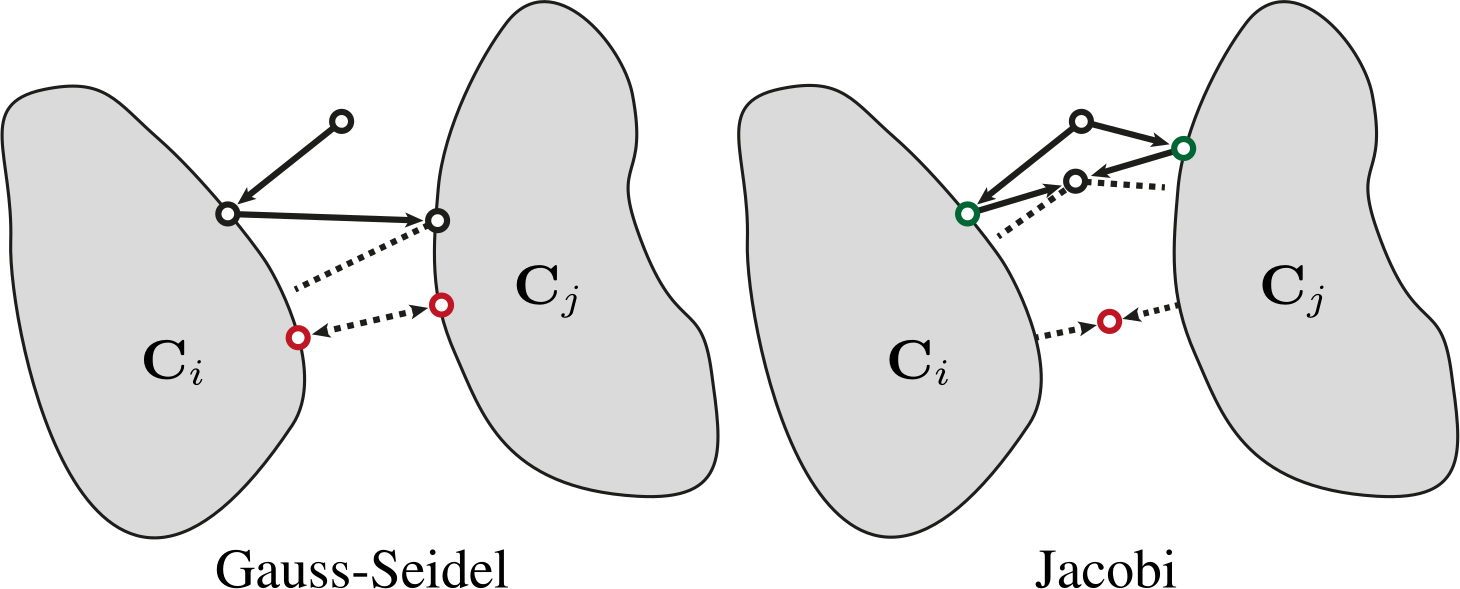
\includegraphics[width = 0.5 \linewidth]{translation/3.png}
  \caption{
    Gauss-Seidel算法与Jacobi算法。PBD中使用的Gauss-Seidel算法会将当前估计值连续投影到每个约束集(本例中为$\vb{C}_i$和$\vb{C}_j$)上。如果没有可行解,即约束集没有重叠,Gauss-Seidel算法就会在不同的约束之间(两个红点之间)摆动。相反,Jacobi算法会将当前估计值并行投影到每个约束集上(绿点),并在第二步折中。这样Jacobi算法就会收敛(红点)。
  }
  \label{fig:translation-3}
\end{figure}

更严重的是,第一步中执行的动量估计也是如此,它包括首先求解方程\eqref{eq:translation-5}中给出的约束。如果将其作为真正的约束添加到优化中,可能会导致完全不兼容的约束集,使收敛性变得更糟。通过首先用初始显式Euler步骤求解动量约束,可以保持整个物体的线性动量,然而,随着优化迭代的时间越长,点的个别动量就会被消除——这与我们提出的隐式Euler求解器建议的在动量和内部弹性之间寻找折中相反(见图~\ref{fig:translation-4})。

\begin{figure}
  \centering
  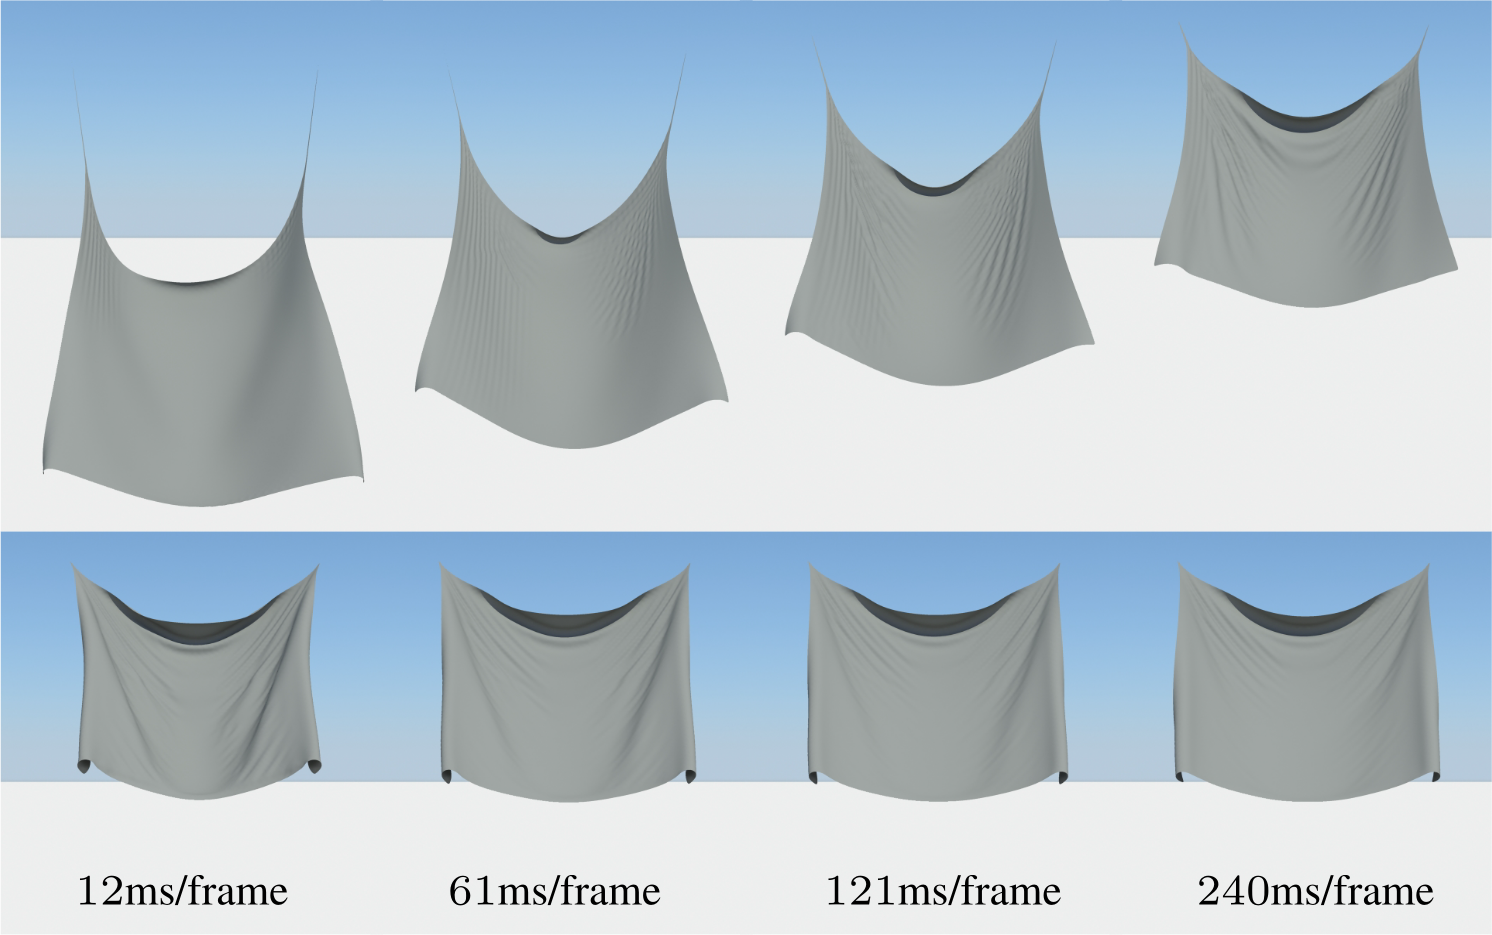
\includegraphics[width = 0.5 \linewidth]{translation/4.png}
  \caption{
    对于一块具有\num{19683}个自由度和\num{19360}个边约束的布料,PBD会根据时间步的允许时间预算显示出不同的材料刚度(上图)。由于额外的动量项和微分坐标表述,即使迭代次数不同,我们的模拟结果也是一致的(下图)。
  }
  \label{fig:translation-4}
\end{figure}

\subsection{Jacobi求解器}

从公式\eqref{eq:translation-11}来看,我们可以通过执行两个步骤以直接的方式求解这些问题。首先,我们用能够处理不兼容约束的Jacobi求解器(见图~\ref{fig:translation-3})替换Gauss-Seidel求解器。一般而言,Jacobi求解器的收敛速度比Gauss-Seidel求解器慢[Thomaszewski et al. 2009]。然而,它们允许使用差分坐标表示法来加快收敛速度,并且能够高效地并行化求解约束投影,从而克服了这一缺点。其次,我们将动量约束引入优化中,以考虑每个点的惯性。正如在连续介质力学视角中看到的,为了实现正确的过程,我们需要通过整合公式\eqref{eq:translation-5}中定义的动量约束项来加回每个点的惯性
\begin{equation}
  \frac{1}{2 h^2} \norm{\vb{M}^{\frac{1}{2}} (\vb{q} - \vb{s}_n)}_F^2 + \sum_i \frac{w_i}{2} \norm{\vb{M}_i^{\frac{1}{2}} (\vb{S}_i \vb{q} - \vb{p}_i)}_F^2 + \delta_{\vb{C}_i}(\vb{p}_i)
  \label{eq:translation-14}
\end{equation}
这样,Jacobi求解器变成了一个两步优化过程:在局部步骤中,首先将当前解$\vb{q}$独立地投影到约束上,通过最小化公式\eqref{eq:translation-11}对所有$\vb{p}_i$进行求解。然后,通过求解关于$\vb{q}$的全局优化,可以在不同解之间达成折中。

\paragraph{与投影隐式Euler法的联系。}

在这一节,我们可以看到这个Jacobi求解器与我们在上一节中介绍的投影隐式求解器程序有多么接近——我们通过选择$\vb{A}_i = \vb{B}_i = \vb{M}_i^{\frac{1}{2}}$来导出这个求解器。通过在下一节中从连续体力学原理导出约束,我们进一步实现了比在PBD中使用的简单基于质量的加权更好的网格剖分独立性和收敛性(见图~\ref{fig:translation-5})。

\begin{figure}
  \centering
  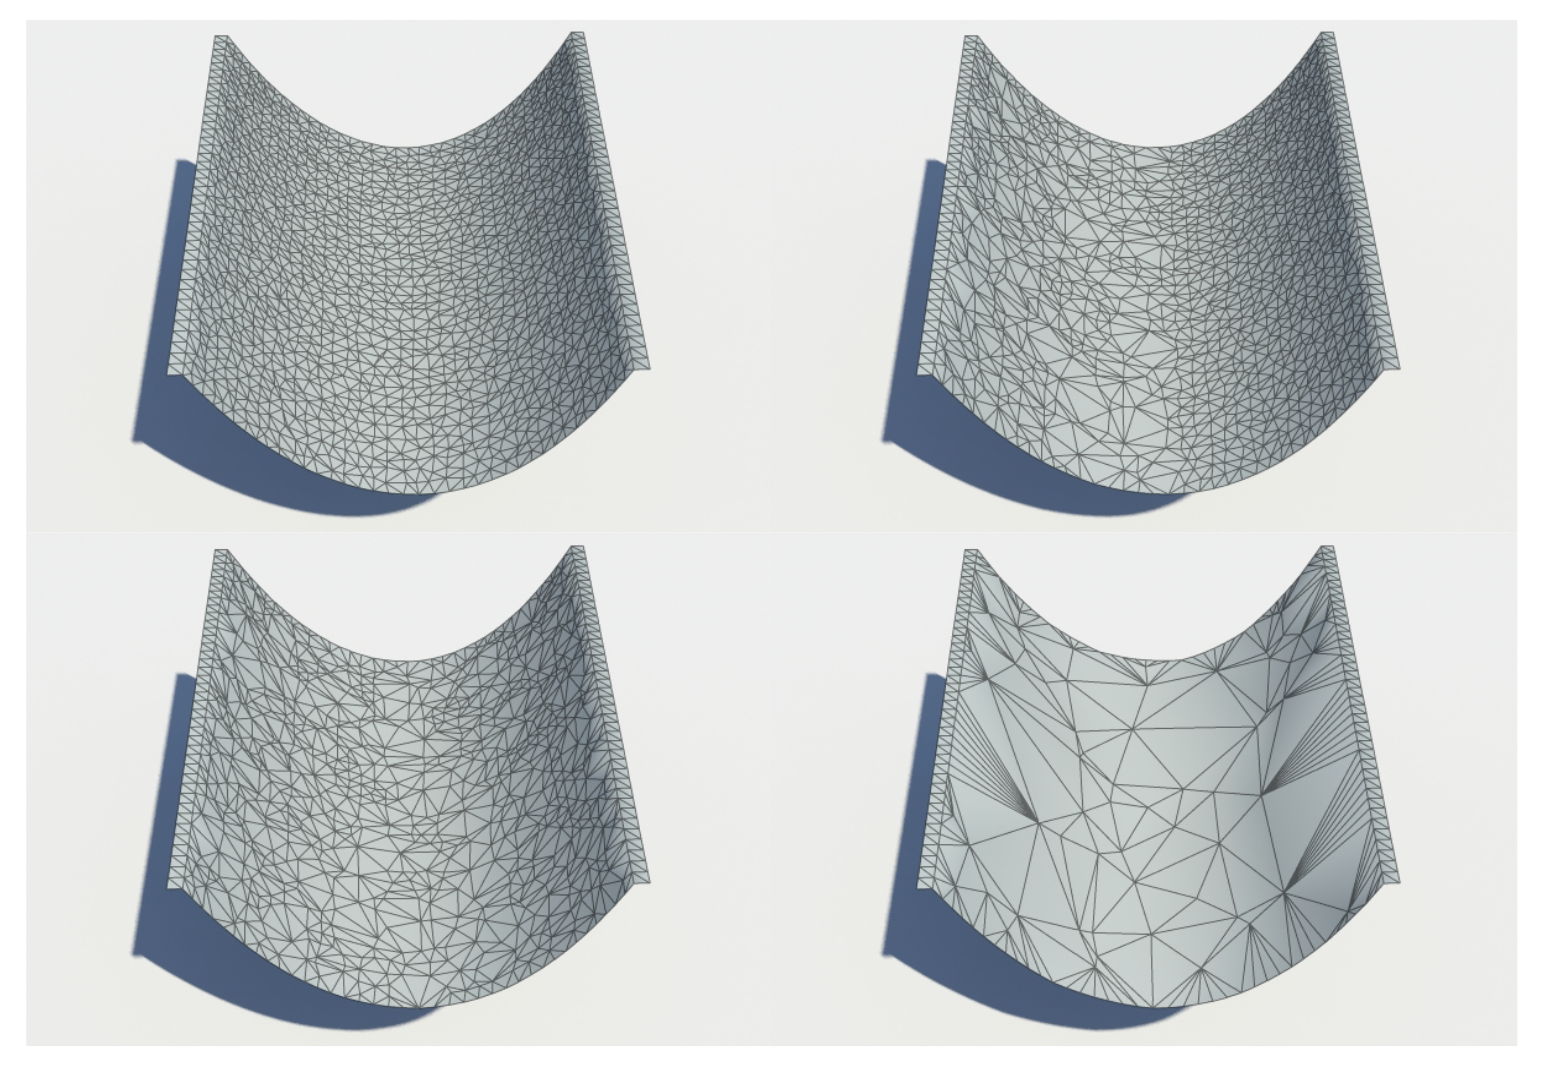
\includegraphics[width = 0.5 \linewidth]{translation/5.png}
  \caption{
    对于给定的连续表面,将我们基于连续性的约束条件离散到不同分辨率的片状简约近似值上,会产生非常相似的定性行为。
  }
  \label{fig:translation-5}
\end{figure}

\section{基于连续介质的约束}
\label{sec:translation-continuum-based-constraints}

微分表示对于我们的局部/全局求解器来提高收敛性是非常重要的。在几何处理中,梯度和Laplace-Beltrami算子在设计高效且鲁棒的模型中扮演着至关重要的角色。在本节中,我们将介绍一组基于这些算子的连续体能量,这些能量允许控制材料在变形过程中的微分属性。我们将展示它们的离散化将具有类似于公式\eqref{eq:translation-7}的形式,这允许在网格细化和非均匀离散化下保持正确的行为。离散势能的局部优化将在附录~\ref{sec:translation-local-solves}中讨论。

\subsection{应力}

\paragraph{连续体能量}

应变能对于模拟可伸展材料至关重要。我们首先讨论2-流形表面,然后将结果扩展到体和曲线。设未变形表面为嵌入$\mathbb{R}^3$中的可微2-流形表面$S$。我们定义未变形表面的分段线性坐标函数为$\vb{g} : S \to \mathbb{R}^3$,及其变形后的对应函数为$\vb{f} : S \to \mathbb{R}^3$。引入一组期望的逐点变换$\vb{T}$ 的集合 $M$,我们构建了一个能量,用以衡量变形和未变形表面之间局部变化的差异,即
\begin{equation}
  E(\vb{f}, \vb{T}) = \frac{w}{2} \int_S \norm{\grad_S{\vb{f}} - \vb{T} \grad_S{\vb{g}}}_F^2 + \delta_M(\vb{T}) \dd{A}
  \label{eq:translation-15}
\end{equation}
其中$\grad_S$是定义在流形表面$S$上的梯度算子。$M$的选择决定了所有允许的静止状态$\vb{T} \grad_S{\vb{g}}$。如果$M$是旋转矩阵集$SO(3)$,我们只是在测量局部偏离刚体运动的程度。在这种情况下,这个能量与Chao等人[2010]提出的变形模型是相同的。如果$M$是具有有界奇异值$\sigma_{\min} < \sigma < \sigma_{\max}$的矩阵集,我们也可以实现类似于Wang等人[2010]的\emph{各向同性应变限制}。这可以进一步扩展到各向异性材料,使用Hernandez等人[2013]提出的参考框架。

\paragraph{离散势能}

如果$S$是一个2-流形单纯复形,这种能量可以通过使用分段线性帽基函数[Botsch et al. 2010]在三角形上离散化。然后,积分被转换为每个三角形势能的求和形式
\begin{equation}
  W(\vb{q}, \vb{T}) = \frac{w}{2} A \norm{\vb{X}_{\vb{f}} \vb{X}_{\vb{g}}^{-1} - \vb{T}}_F^2 + \delta_M(\vb{T})
  \label{eq:translation-16}
\end{equation}
其中$A$是三角形面积,$\vb{X}_{\vb{f}} = [\vb{q}_j - \vb{q}_i, \vb{q}_k - \vb{q}_i] \in \mathbb{R}^{2 \times 2}$包含当前状态中保距嵌入2D的三角形边,类似地$\vb{X}_{\vb{g}}$包含静止状态的三角形边。注意,这个离散势能的形式与公式\eqref{eq:translation-7}中的形式相同,其中$\vb{A}$是静止状态边和面积的函数,而$\vb{B}$仅依赖于静止状态的面积。图~\ref{fig:translation-6}展示了应用于窗帘示例的应变限制约束。

\begin{figure}
  \centering
  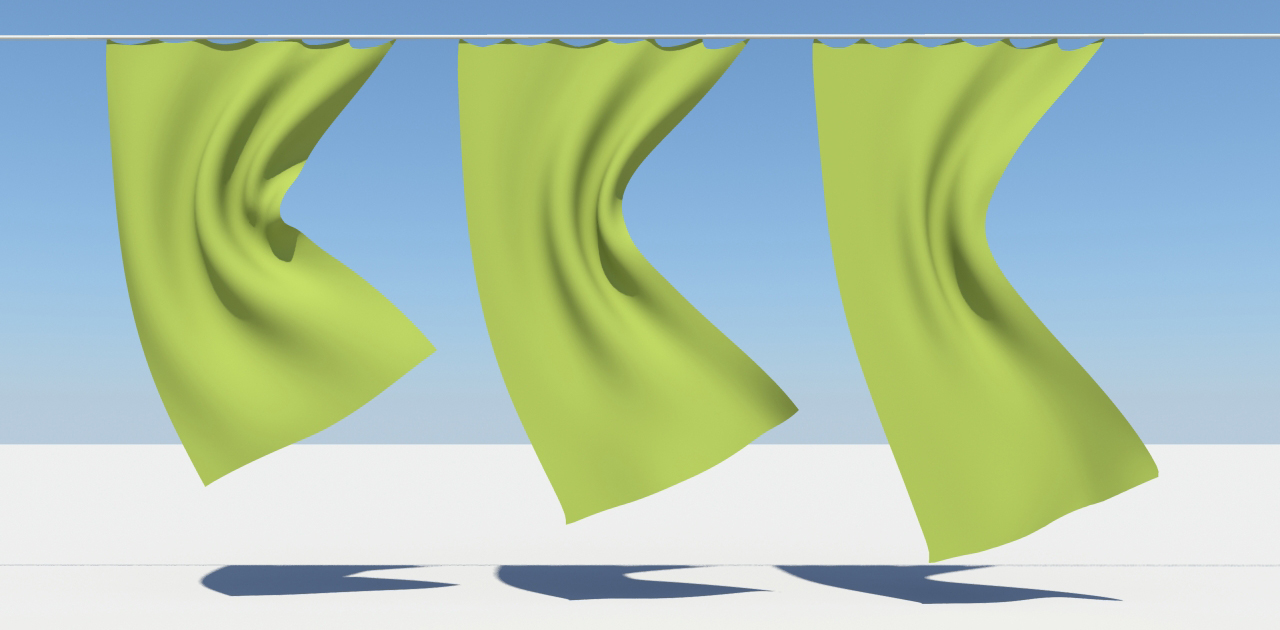
\includegraphics[width = 0.5 \linewidth]{translation/6.png}
  \caption{
    从相同的网格开始,应变限制可以模拟可以承受小到中等程度拉伸的材料。从左到右,我们使用的应变限制分别为$[\SI{-10}{\percent}, \SI{+10}{\percent}]$、$[\SI{-20}{\percent}, \SI{+20}{\percent}]$和$[\SI{-30}{\percent}, \SI{+30}{\percent}]$。请注意,当极限值增加时,布会如何拉伸以及褶皱如何被吸收。
  }
  \label{fig:translation-6}
\end{figure}

\paragraph{体和曲线。}

体的势能可以以类似的方式定义:如果$S$是一个3-流形单纯复形,能量可以通过替换三角形的面积为四面体的体积,并且有$3 \times 3$边矩阵来离散化。注意,如果我们对这种能量在一组边上进行1D离散化,我们会得到一个类似于Liu et al.[2013]的快速模拟质量弹簧模型,在此基础上,边势能已经基于边长度适当加权。

\subsection{面积和体积保持约束}

在模拟不可压缩材料时,面积和体积的不变是非常重要的。使用公式\eqref{eq:translation-15}的连续体能量,我们可以定义$M$为具有有界行列式的矩阵集合$\sigma_{\min} < \det(\vb{T}) < \sigma_{\max}$,有效地使我们能够控制体积变化的量。如果$\sigma_{\min} < 1$,则模拟的材料允许压缩;类似地,如果$\sigma_{\max} > 1$,则材料允许膨胀。图~\ref{fig:translation-7}展示了体积保持约束和应变约束的结合。

\begin{figure}
  \centering
  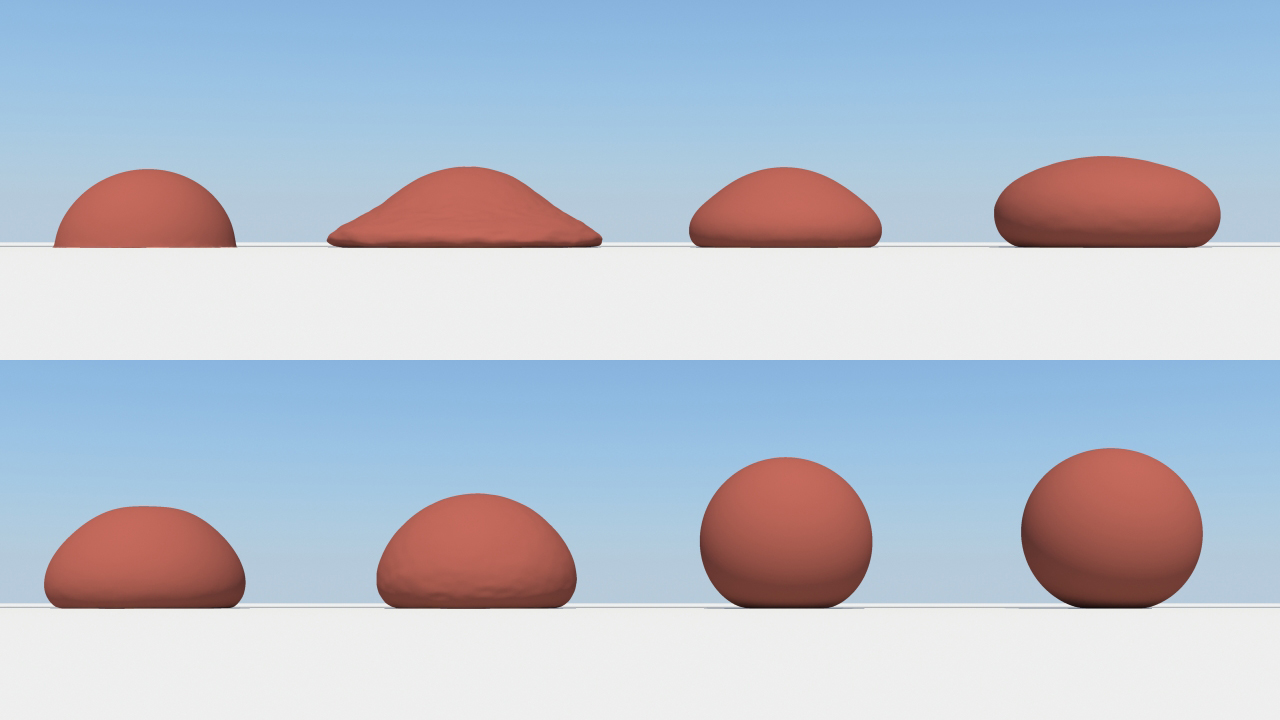
\includegraphics[width = 0.5 \linewidth]{translation/7.png}
  \caption{
    通过不同重量的体积保持约束和应变约束组合,可以模拟不同类型的体积物体材料。
  }
  \label{fig:translation-7}
\end{figure}

\subsection{基于范例的仿真}

基于范例的仿真允许通过提供一些材料应该遵循的变形范例来模拟艺术性的弹性材料行为[Martin et al. 2011; Koyama et al. 2012; Jones et al. 2013]。我们使用一个与公式\eqref{eq:translation-15}类似的能量,定义在3-流形表面上,如下所示:
\begin{equation}
  E(\vb{f}, \vb{R}, \vb{w}) = \frac{w}{2} \int_S \norm{\grad_S{\vb{f}} - \vb{R} \grad_S{\vb{h}(\vb{w})}}_F^2 + \delta_{SO(3)}(\vb{R}) \dd{V}
  \label{eq:translation-17}
\end{equation}
其中$\vb{h}(\vb{w})$是由范例定义的参数化的静止形状。我们将静止形状表述为$\vb{h}(\vb{w}) = \vb{g} + \sum_i w_i(\vb{R}_i \vb{g}_i - \vb{g})$,其中$\vb{g}_i$定义为范例的分段线性坐标函数,$\vb{R}_i$是预先计算的旋转矩阵,逐点定义,使其局部旋转$\vb{g}_i$以最佳对齐未变形状态$\vb{g}$,这与Koyama et al.[2012]的思想相似。

我们可以使用分段线性帽基函数离散化这个连续体能量,导出每个四面体的势能之和
\begin{equation}
  W(\vb{q}, \vb{R}, \vb{w}) = \frac{w}{2} V \norm{\vb{X}_{\vb{f}} \vb{X}_{\vb{g}}^{-1} - \vb{R} \vb{X}_{\vb{h}}(\vb{w}) \vb{X}_{\vb{g}}^{-1}}_F^2 + \delta_{SO(3)}(\vb{R})
  \label{eq:translation-18}
\end{equation}
其中$\vb{X}_{\vb{h}}(\vb{w}) = \vb{X}_{\vb{g}} + \sum_i w_i(\vb{R}_i \vb{X}_{\vb{g}_i} - \vb{X}_{\vb{g}}$)。请注意,范例权重$\vb{w}$可以在每个元素上局部定义,也可以全局定义,分别导致局部或全局的变形耦合。在图~\ref{fig:translation-8}中可以找到使用此约束的三辆相撞汽车的范例。

\begin{figure}
  \centering
  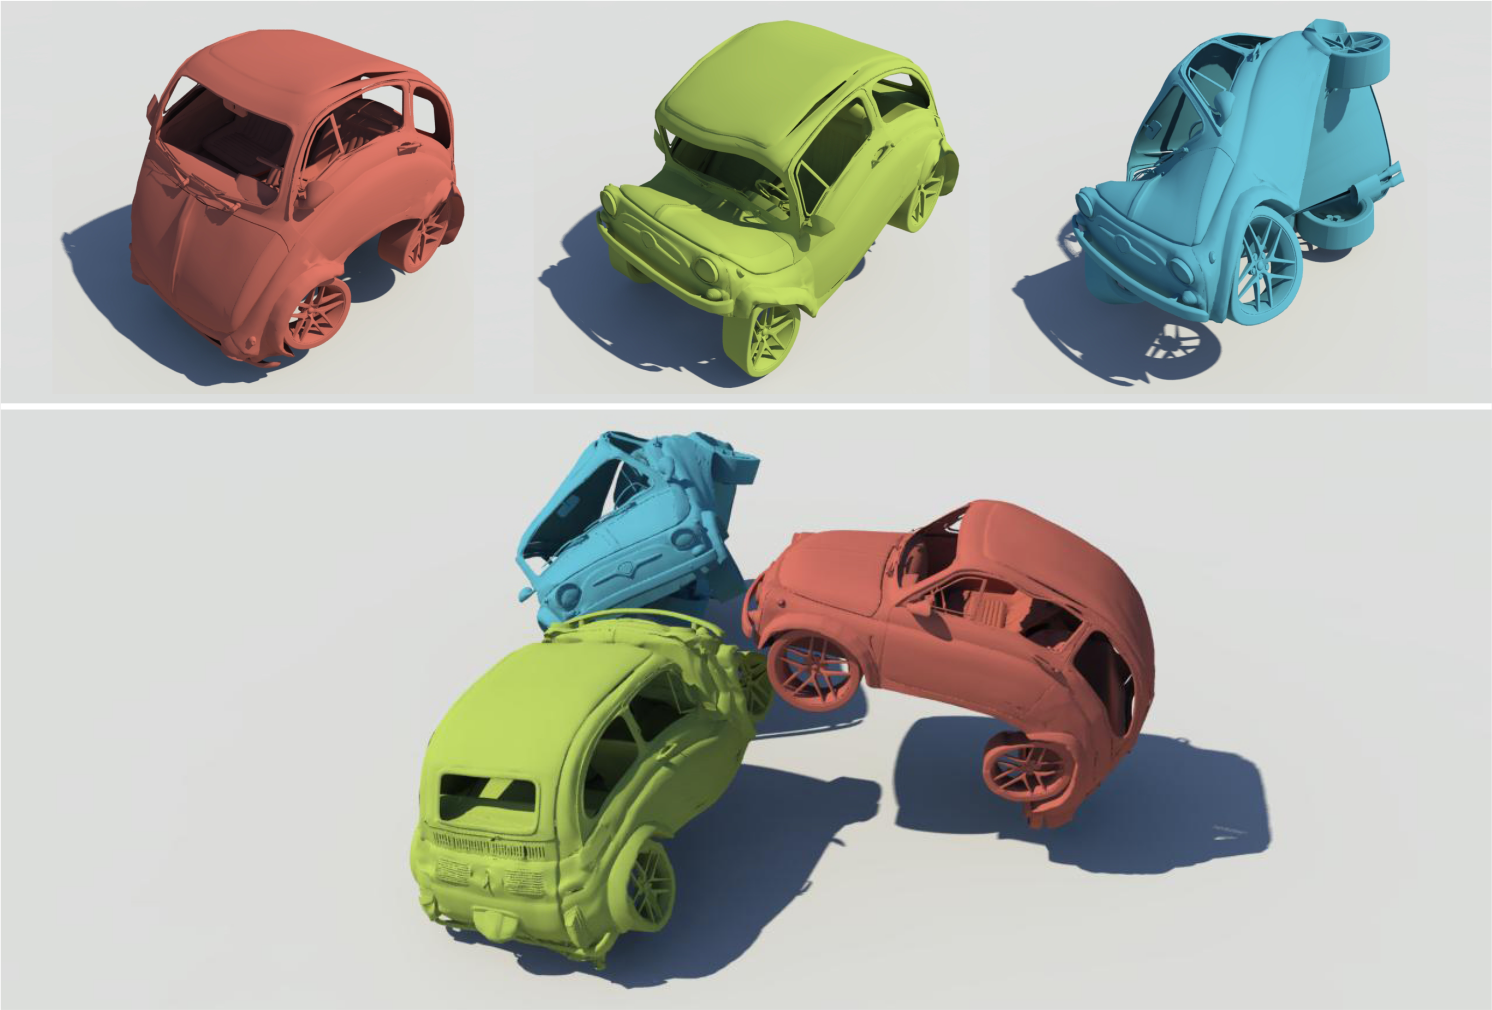
\includegraphics[width = 0.5 \linewidth]{translation/8.png}
  \caption{
    使用基于范例的约束将变形范例(上图)添加到模拟中,可以模拟复杂的艺术材料。在这个场景中,三辆汽车相撞,并按照规定的范例(下图)以卡通的方式作出反应。
  }
  \label{fig:translation-8}
\end{figure}

\subsection{弯曲}

\paragraph{连续体能量。}

薄壳和薄板通常使用基于边缘横跨角度的弯曲能进行模拟[Grinspun et al. 2003]。更近期地,已经提出了高效的模型来模拟不可伸展表面的弯曲,这些模型将Laplace-Beltrami算子与平均曲率法向量联系起来[Bergou et al. 2006; Garg et al. 2007]。我们引入了一个测量绝对平均曲率平方差的弯曲能
\begin{equation}
  E(\vb{f}) = \frac{w}{2} \int_S \pqty{\abs{H_{\vb{f}}} - \abs{H_{\vb{g}}}}^2 \dd{A}
  \label{eq:translation-19}
\end{equation}
其中$H_{\vb{f}}$ 和 $H_{\vb{g}}$分别是变形和未变形表面的平均曲率函数。对于等距变形(不可伸展表面),我们可以使用辅助旋转矩阵重写能量为
\begin{equation}
  E(\vb{f}, \vb{R}) = \frac{w}{2} \int_S \norm{\Delta_S{\vb{f}} - \vb{R} \Delta_S{\vb{g}}}_F^2 + \delta_{SO(3)}(\vb{R}) \dd{A}
  \label{eq:translation-20}
\end{equation}
其中$\Delta_S$是定义在流形表面$S$上的Laplace-Beltrami算子。这是因为平均曲率向量等于应用于坐标函数的表面的Laplace-Beltrami算子。对于等距变形,Laplace-Beltrami算子不会改变,因此可以在未变形表面上定义。请注意公式\eqref{eq:translation-20}与公式\eqref{eq:translation-15}是多么相似,将梯度替换为Laplace-Beltrami算子。因此,将应变限制和基于范例的概念应用于弯曲能也是有可能的。

\paragraph{离散势能}

如果$S$是一个2维单纯复形,公式\eqref{eq:translation-20}可以使用分段线性帽函数基进行离散化,从而得到每个顶点的势能形式为
\begin{equation}
  W(\vb{q}, \vb{R}) = \frac{w}{2} A \norm{\vb{X}_{\vb{f}} \vb{c} - \vb{R} \vb{X}_{\vb{g}} \vb{c}}_2^2 + \delta_{SO(3)}(\vb{R})
  \label{eq:translation-21}
\end{equation}
其中$A$是顶点的Voronoi面积,$\vb{X}_{\vb{f}}$和$\vb{X}_{\vb{g}}$分别包含了顶点在当前配置和静止配置下的一环边。向量$\vb{c}$存储了除以Voronoi面积的共同余切权重[Botsch et al. 2010]。图~\ref{fig:translation-9}中展示了一个弯曲约束的例子。如附录中所示,这种弯曲约束允许非常高效的局部求解,因为它可以仅仅通过对变形配置的平均曲率向量进行简单的归一化来实现。

\begin{figure}
  \centering
  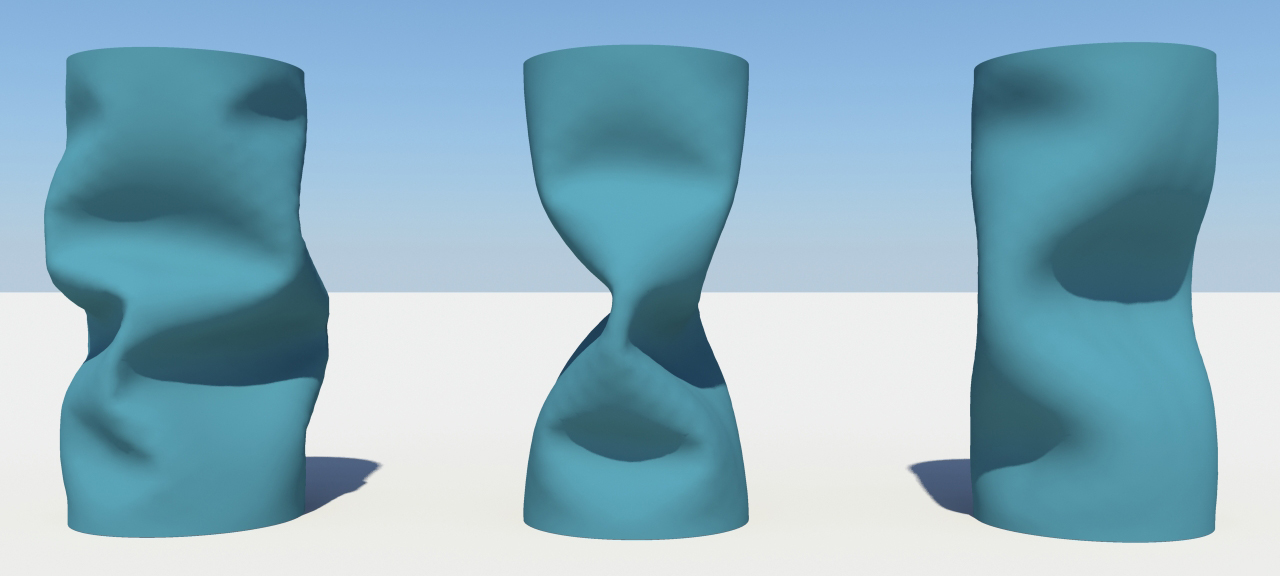
\includegraphics[width = 0.5 \linewidth]{translation/9.png}
  \caption{利用从左到右递增的弯曲重量模拟薄壳圆柱体。当圆柱体受到压缩时,会出现不同频率的屈曲模式。}
  \label{fig:translation-9}
\end{figure}

\section{离散约束}

上一节中从连续体能量导出的约束允许我们模拟多种多样的弹性体。对于实际的动画系统来说,其他约束同样重要。我们直接将这些约束建模为离散约束。

\paragraph{位置约束。}

如前所述,可以通过在公式\eqref{eq:translation-7}中简单选择$\vb{A}_i = \vb{B}_i = \vb{I}$来直接约束单个自由度。然后,可以通过定义约束集为期望的目标位置来实现\emph{Dirichlet边界条件},以便固定对象或创建可交互锚点。

\paragraph{碰撞。}

以隐式方式处理碰撞天然适合于我们的通用求解器中,并且允许在碰撞解决过程中尊重动量平衡和内部约束。当检测到碰撞时,我们动态地添加新的单侧平面约束。对于位置约束,我们再次在公式\eqref{eq:translation-7}中选择$\vb{A}_i = \vb{B}_i = \vb{I}$。对于发生碰撞的点$\vb{q}_c$,我们首先找到最近的表面点$\vb{b}$和法向$\vb{n}$,定义一个碰撞平面,使得约束集$\vb{C}$定义为半空间$\vb{n}^T (\vb{q} - \vb{b}) \geqslant 0$。在局部步骤中,投影到这个半空间是平凡的,因为它要么是一个平面投影,要么是恒等映射。请注意,单向定义碰撞约束允许我们克服在隐式碰撞处理中常见的粘附问题。类似于PBD,我们通过在更新速度时改变碰撞顶点的速度来处理摩擦和恢复力。一个简单的阻尼模型也可以通过过滤速度来实现[Müller et al. 2007]。

\paragraph{更多约束。}

一般类型的几何约束,例如使用铰链角度的弯曲约束[Bender et al. 2013],可以轻松地并入到我们的求解器中。局部求解可以通过最小化公式\eqref{eq:translation-7}来通用地执行,通过辅助变量。对于许多几何约束,可以找到这种最小化的封闭形式解[Bouaziz et al. 2012]。如果不存在封闭形式解,优化可以使用序列二次规划(SQP)[Nocedal and Wright 2006]来解决。如第~\ref{sec:translation-gauss-seidel-solver}节所示,对于$\vb{A} = \vb{B} = \vb{M}^{\frac{1}{2}}$的情况,SQP的一步与PBD更新类似[Bender et al. 2013]。

\section{实验结果}

\subsection{通用性}

我们的求解器不依赖于任何特定类型的约束,并且能够在相同的设置中处理各种各样的几何约束,这使得使用单一求解器模拟复杂场景成为可能,并且还能以隐式的方式鲁棒地处理对象间的交互作用。在图~\ref{fig:translation-1}中,我们展示了一个包含不同约束类型的复杂场景,其中的对象也是相互耦合的。例如,树和房子是用体积应变约束来建模的,而晾衣绳、布料、草和树叶则使用边缘应变和弯曲约束。

\paragraph{衣物和壳体。}

在图~\ref{fig:translation-10}中,我们简单地使用边缘应变约束来模拟海盗旗的行为。风力作为风向和三角形法线的函数被添加。当风力过强时,海盗旗会被撕裂。这是通过在应变超过一定阈值时移除边缘约束来实现的。可以使用限制三角形应变结合弯曲约束来模拟可以承受小到中等程度拉伸的更复杂的布料(见图~\ref{fig:translation-6})。通过改变应变和弯曲约束的权重,可以模拟其他类型的材料,如薄板和薄壳。在图~\ref{fig:translation-9}中,我们可以看到一个从顶部压缩的薄圆柱体,由于应变和弯曲约束刚度比例的不同,展现出不同的屈曲模式。

\begin{figure}
  \centering
  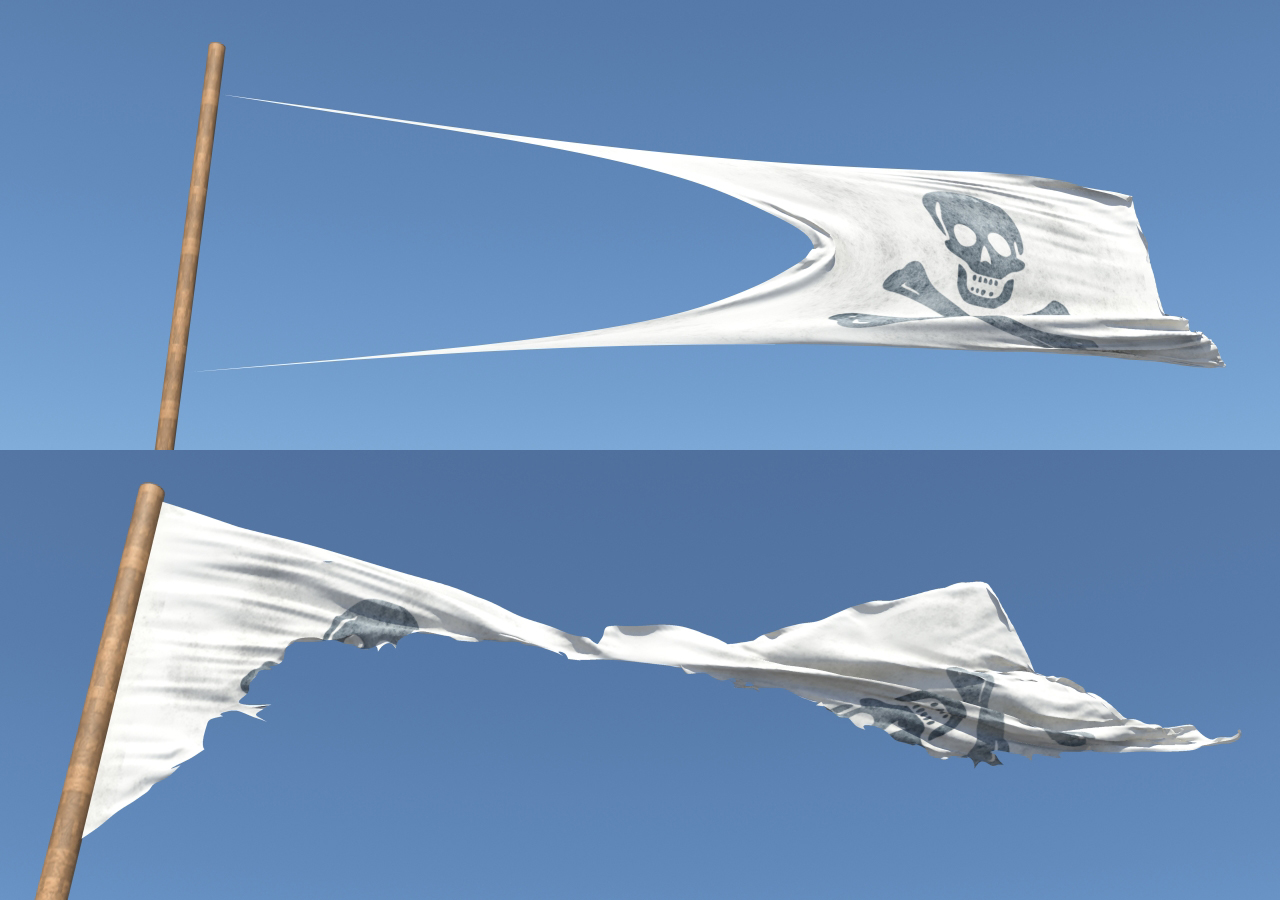
\includegraphics[width = 0.5 \linewidth]{translation/10.png}
  \caption{
    即使在极端风力作用下,我们的投影隐式求解器仍然保持稳定。求解器在每次迭代中弱化能量,使得任何安全措施都变得不必要(上图)。海盗旗在实时中被风撕裂,使用动态更新的约束(下图)。
  }
  \label{fig:translation-10}
\end{figure}

\paragraph{固体和基于范例的模拟。}

我们通过在四面体网格上应用应变和体积约束来模拟固体。如图~\ref{fig:translation-7}所示,不同类型的材料应变约束在我们的局部/全局求解器中进行了1次、10次和20次迭代模拟。值得注意的是,仅经过10次迭代,我们的方法看起来与使用牛顿法计算的收敛解非常相似,但计算成本只是一小部分。

通过改变这些约束的权重组合可以模拟不同的材料。虽然我们不能模拟任意的非线性材料,但我们能够通过结合弱应变约束和更强的限制应变约束来近似一些非线性行为。然后,当材料小变形时是柔软的,而当变形达到应变限制时,第二个约束变得活跃(见随附视频)——这是非线性材料模型通常模拟的行为。结合不同的二次势能已经在[Harmon et al. 2009]中用于碰撞处理,但也非常适合我们的框架来模拟非线性材料行为。

我们的公式也可以用于基于范例的体积网格模拟。这允许对物理模拟进行艺术性控制。在图~\ref{fig:translation-8}中,三辆汽车在碰撞后以卡通化的方式根据输入范例变形。类似于[Martin et al. 2011],汽车表面被嵌入到体积网格中,然后使用我们的求解器进行变形。

\subsection{鲁棒性和简单性}

我们方法的一个重要优势是数值稳定性。在图~\ref{fig:translation-10}中,我们展示了即使在极端力的作用下,我们的求解器也能保持鲁棒。同样地,我们的方法在网格元素退化的情况下也能保持可靠。这一点可以在压缩在两个平面之间的球体的模拟中看到(参见随附视频)。我们方法的唯一要求是输入模型的网格元素必须表现良好,以便计算原始流形的梯度和Laplace-Beltrami算子的离散化。

我们通过在算法~\ref{alg:translation-1}中展示我们的优化过程来说明我们方法的简单性。通过移除第~\ref{alg:translation-1L7}行并在第~\ref{alg:translation-1L5}行中将$\vb{p}_i$改为$\vb{q}_{n + 1}$,我们能够完全恢复原始PBD算法[Müller et al. 2007]的结构。此外,注意到引入一个新的约束只需要定义在局部求解中使用的约束投影(如果已知则为精确的,如果不知道则为[Müller et al. 2007]中给出的一般近似投影方案)以及适当的二次距离度量(矩阵$\vb{A}_i$和$\vb{B}_i$)的定义。

\subsection{准确性与性能}

\paragraph{与牛顿法的比较。}

在图~\ref{fig:translation-12}中,我们比较了我们的局部/全局求解器与牛顿法在求解公式\eqref{eq:translation-15}的离散化时的性能,其中$M = SO(3)$,类似于[Chao et al. 2010]。如图~\ref{fig:translation-12}所示,局部/全局方法在迭代次数上收敛得更慢。这是完全合理的,因为牛顿法表现出二次收敛,而局部/全局求解器(块坐标下降法)具有线性收敛。然而,当我们从计算时间的角度来看收敛性时,我们注意到我们的方法对于交互式应用来说比牛顿法更快。大约30次局部/全局迭代可以在1次牛顿迭代的时间内完成。这是因为在每次牛顿迭代中都需要重新计算Hessian矩阵,因此需要解一个新的线性系统。

此外,在图~\ref{fig:translation-11}和随附的视频中,我们观察到大约10次迭代后,模拟的效果在视觉上与使用牛顿法收敛的结果相似,这使得我们的方案成为实时应用的更好选择,其中高精度不是主要关注点。在几何处理和模拟中使用的一些先前的局部/全局求解器已经观察到了这种行为[Myles and Zorin 2012; Liu et al. 2013]。注意,对于第~\ref{sec:translation-continuum-based-constraints}节中提出的连续体能量实现牛顿法并非易事,因为需要对SVD[McAdams et al. 2011]进行微分,并且在每个时间步都需要计算新的Hessian矩阵。此外,优化中需要集成一些保护措施,因为Hessian矩阵可能变得不定,还需要一个线搜索过程来避免超调。

\begin{figure}
  \centering
  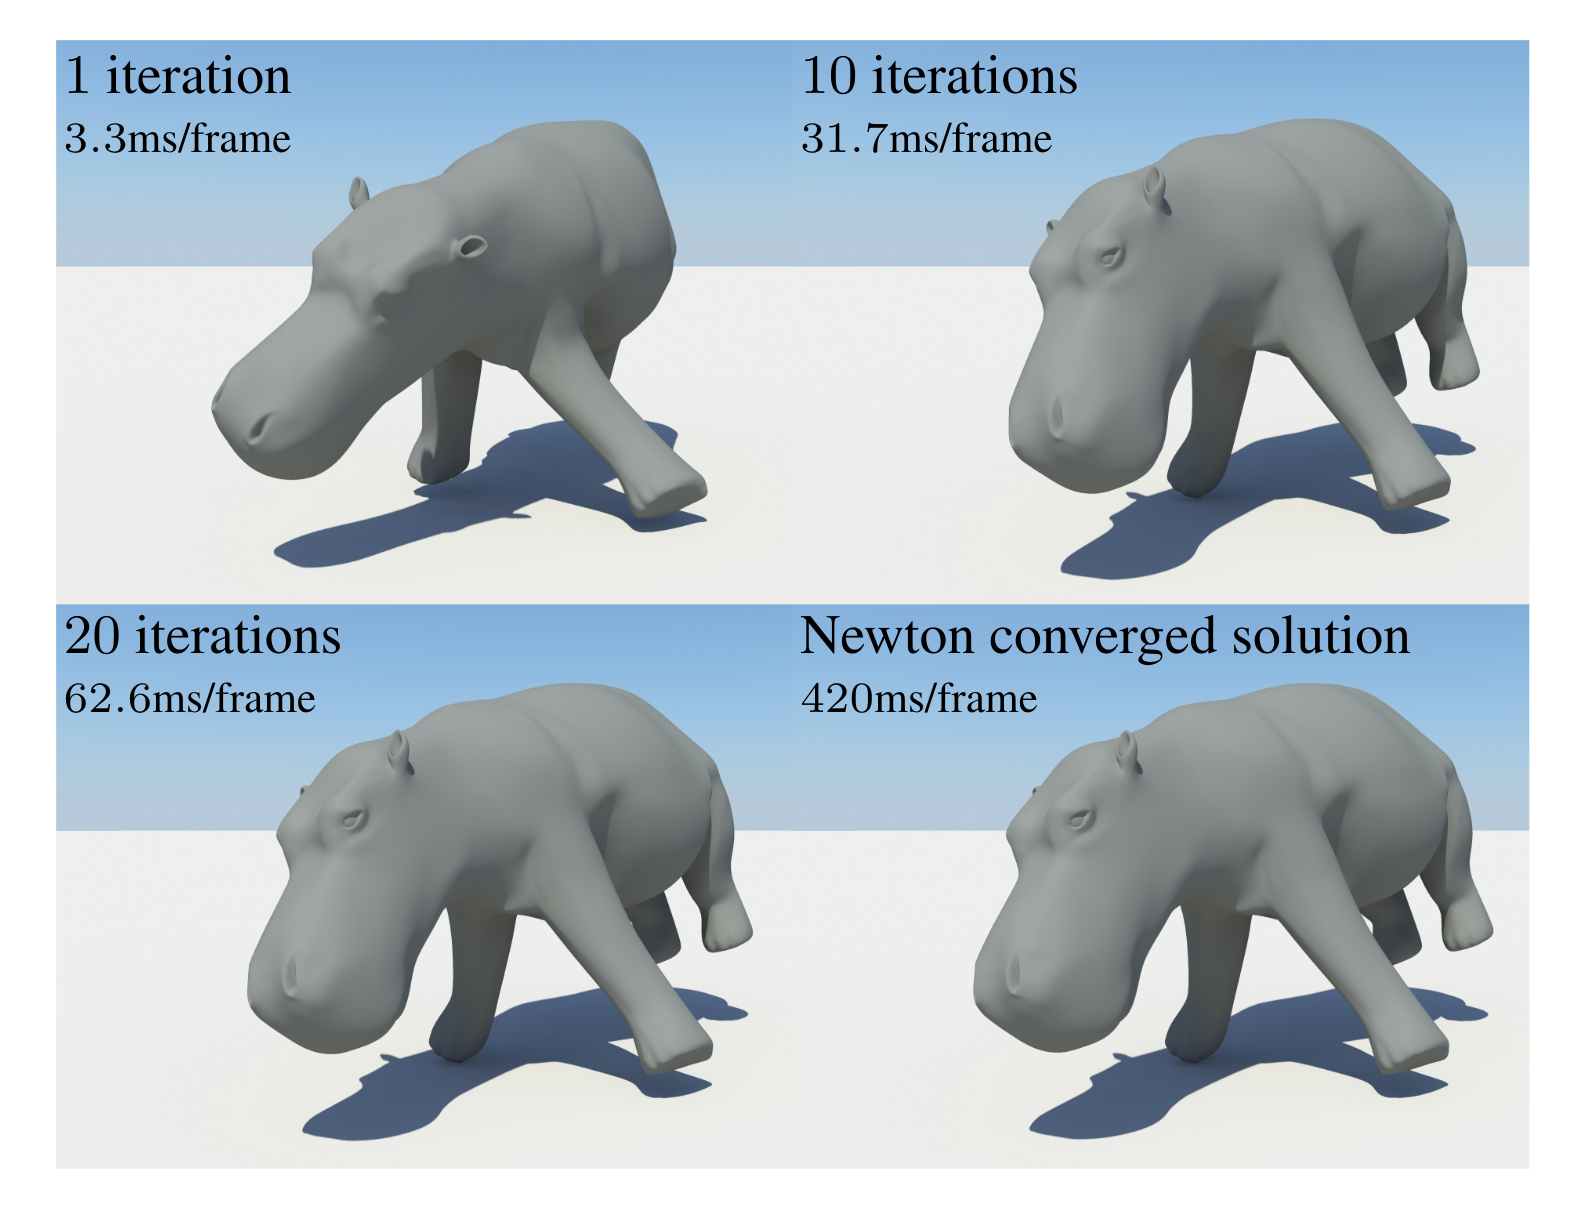
\includegraphics[width = 0.5 \linewidth]{translation/11.png}
  \caption{
    我们使用局部/全局求解器对这只具有\num{7161}个自由度和\num{8406}个应变约束的体积河马进行了1、10和20次迭代模拟。有趣的是,经过10次迭代后,我们的方法与使用牛顿法计算出的收敛解非常相似,而计算成本仅为牛顿法的一小部分。
  }
  \label{fig:translation-11}
\end{figure}

\begin{figure}
  \centering
  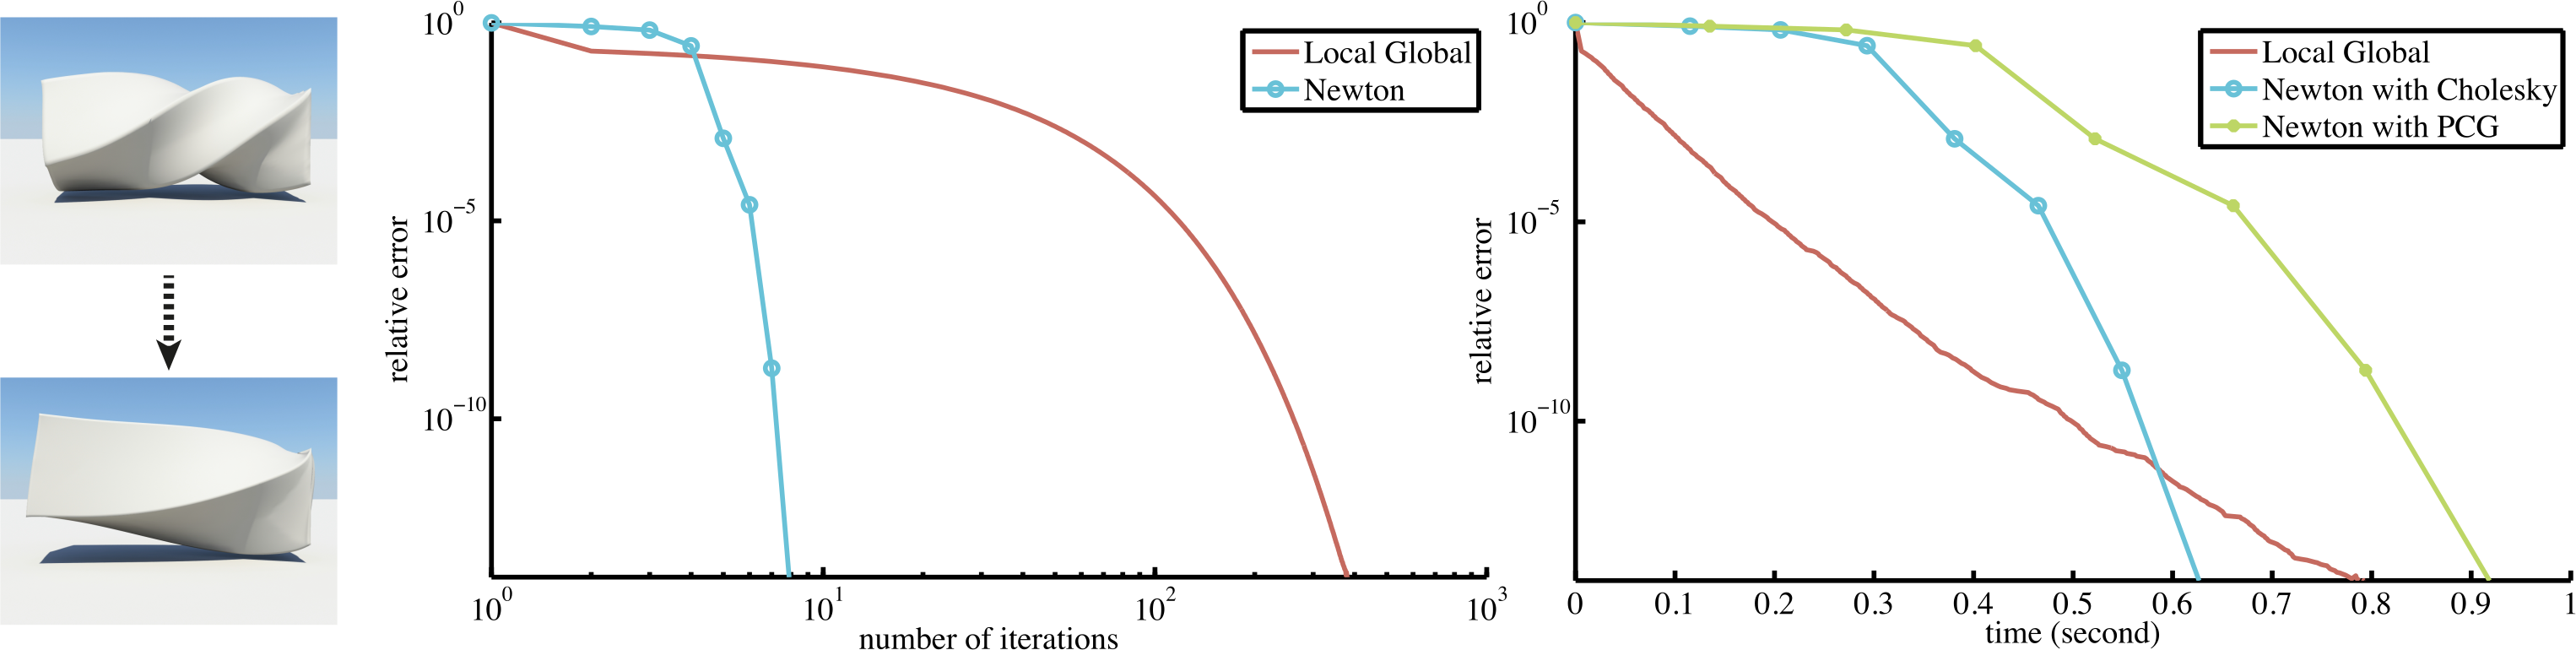
\includegraphics[width = \linewidth]{translation/12.png}
  \caption{
    通过比较相对误差随迭代次数的减少,我们观察到牛顿法比我们的局部/全局方法收敛得更快。然而,这并不反映每次迭代的成本,因为每次牛顿迭代都需要求解一个变化的线性系统。观察相对误差随计算时间的减少,我们注意到我们的局部/全局方法在相对误差达到\num{e-10}时表现出更好的性能,这使得我们的方法对于交互式应用特别有吸引力。在这些曲线中,相对误差定义为相对于最优解的归一化误差$(\epsilon(\vb{q}_i) - \epsilon(q*)) / (\epsilon(\vb{q}_0) - \epsilon(\vb{q}^*))$,并且是针对一个扭曲条例子(左)进行测量的,该例子具有\num{4290}个自由度和\num{4099}个四面体应变约束。
  }
  \label{fig:translation-12}
\end{figure}

\paragraph{与基于位置的动力学的比较。}

我们还将我们的方法与使用边应变约束的PBD进行了比较。如第~\ref{sec:translation-position-based-dynamics-view}节所解释的,PBD不包括动量约束,这使得材料刚度依赖于迭代次数。这可以在随附的视频和图~\ref{fig:translation-4}中看到,对于不同数量的迭代,PBD模拟的材料刚度发生了巨大变化。而在我们的方法中,材料刚度与迭代次数的依赖性要小得多。

\paragraph{网格独立性}

在第~\ref{sec:translation-continuum-based-constraints}节中,我们提出了一组从连续体能量中派生出的新约束。如图~\ref{fig:translation-5}所示,这些新约束允许我们的求解器在不同的分片单纯形近似同一底层表面的情况下,保持变形行为的一致性。这对于计算机图形应用和交互式环境来说是一个重要的特性,因为在开发过程中网格分辨率可能会频繁变化,而且为了提高性能,广泛使用几何细节层次。PBD方法缺乏收敛性,由于材料行为依赖于底层网格和迭代次数的数量,这使得正确处理几何细节层次变得困难[Häggström 2009]。

\section{实现}

本文提出的完整框架是用C++实现的。我们使用OpenMP来并行化局部步骤,并且通过预先对线性系统进行稀疏Cholesky分解,然后并行地对$x$、$y$和$z$坐标进行三次回代,从而并行解决全局步骤。动态约束通过对线性系统进行秩的更新和降级来处理。我们使用Eigen库(eigen.tuxfamily.org)进行密集和稀疏的线性代数计算。我们使用标准的单纯形质量离散化[Hughes 2000]或其集中版本来计算质量矩阵,两者之间没有明显差异。

\paragraph{计时。}

对于中等大小模型的模拟(\SI{< 30}{k}约束和\SI{< 30}{k}自由度),通常\numrange{5}{10}次迭代就足够了。每次迭代\qtyrange{1}{6}{\milli\second},这使得在MacBook Pro 2.7 GHz Intel Quad-core i7处理器和16GB内存的电脑上能够实现实时模拟。关于计时和网格的统计数据可以在随附的视频中找到。此外,随附的应用程序展示了在多个示例上的性能表现。

\section{局限与未来工作}

尽管我们的隐式Euler求解器既高效又稳健,但它表现出隐式阻尼效应。在不久的将来,我们计划将我们的方法扩展到辛积分器[Kharevych et al. 2006],这些积分器提供更好的能量行为。当优化提前终止时,也可以观察到阻尼现象。这是因为如果优化没有运行足够的迭代次数,外部力可能无法完全通过网格传播。在大型网格中,这种效应更加明显,因为需要更多的迭代才能收敛。作为未来的工作,我们希望通过实现我们代码的GPU版本来提高求解器的速度,并专注于拓扑变化(切割、断裂)导致的动态变化约束。虽然在GPU上解决局部步骤仍然简单,但全局系统正在变化,使得高效解决它变得更加复杂。如果我们想将我们的方法扩展到类似[Macklin and Müller 2013]的流体模拟,那么这个问题会变得更加突出,因为邻域关系总是在变化。

我们为了简单和效率而牺牲了硬约束。以柔性方式处理所有约束,使我们能够以统一且有效的方式处理它们。然而,在某些情况下,能够强制执行硬约束,例如用于碰撞处理或边界条件,将是有利的。硬约束仍然可以通过增加约束的权重来近似。然而,这可能会降低线性系统的条件,并可能导致锁定伪影。

另一个有趣的进一步研究领域是扩大我们的约束集。我们想要探索的一个方向是模拟更复杂的变形行为,如各向异性和非线性材料。此外,将刚体集成到同一模拟框架中也将是有吸引力的。

\section{结论}

我们引入了一种新的基于隐式约束的求解器,用于实时模拟。我们的方法基于物理系统的抽象、基于约束的描述,使得我们的方法在用于模拟各种不同几何形状和材料方面具有普遍性。为了解决约束问题,我们应用了一个局部/全局求解器,它保证能够弱化地降低能量,从而无需任何安全保护措施,赋予了我们的方法以鲁棒性。我们简单的基于约束的公式只需要为给定的约束定义一个投影算子(局部求解),这使得它非常容易实现,并且很容易将新模型引入求解器。此外,全局求解只需要求解一个线性系统,如果约束数量保持不变,那么系统矩阵是常数,从而导致高效的计算。由于局部求解的独立性,这种方法也非常适合并行处理,进一步提升了性能。我们从连续体能量直接导出了一系列广泛的约束,通过适当的离散化使得求解器对于具有不同分辨率的非均匀网格化具有鲁棒性。考虑到这些特点,我们相信我们的方法在基于位置的模拟的简单性、通用性、鲁棒性和性能以及连续介质力学的严谨性和准确性之间取得了正确的平衡。我们认为这使得我们的方法适用于计算机图形学中许多实时和离线模拟的应用。

\paragraph{致谢。}

我们感谢James O'Brien、Adam Bargteil、Basil Fierz和Bernhard Thomaszewski的深入讨论以及审稿人的宝贵意见。我们感谢\emph{luismigabril}提供卡通房屋模型,感谢Daniel Grauer制作预告场景模型。我们还要感谢尤利-施瓦茨堡(Yuliy Schwartzburg)为配乐视频所做的解说。本研究得到了瑞士国家科学基金会20PA21L 129607号基金、欧盟第七框架计划(FP/20072013)/ERC补助金协议n. 257453: COSYM下的欧洲研究理事会以及美国国家科学基金会IIS-1350330 Career Award的支持。

\appendix

\section{局部求解}
\label{sec:translation-local-solves}

% 附录的内容。

\paragraph{应变。}

在局部步骤中,固定$\vb{q}$最小化$\vb{T}$时
\begin{equation}
  \min_{\vb{T}} \norm{\vb{X}_{\vb{f}} \vb{X}_{\vb{g}}^{-1} - \vb{T}}_F^2 + \delta_M(\vb{T})
  \label{eq:translation-22}
\end{equation}
该优化可以重新表述为
\begin{equation}
  \min_{\Sigma^*} \norm{\Sigma - \Sigma^*}_F^2 \qq{s.t.} \sigma_{\min} < \Sigma_{ii}^* < \sigma_{\max}
  \label{eq:translation-23}
\end{equation}
其中$\vb{X}_{\vb{f}} \vb{X}_{\vb{g}}^{-1} = \vb{U} \Sigma \vb{V}^T$ 且 $\vb{T} = \vb{U} \Sigma^* \vb{V}^T$。最优解可以计算为$\Sigma^*$,即将奇异值$\Sigma$限制在$\sigma_{\min}$和$\sigma_{\max}$之间。对于四面体,如果$\det(\vb{X}_{\vb{f}} \vb{X}_{\vb{g}}^{-1}) < 0$,则最后一个奇异值取反,以避免反射。

\paragraph{面积和体积。}

与应变约束类似,体积约束的局部最小化可以重新表述为
\begin{equation}
  \min_{\Sigma^*} \norm{\Sigma - \Sigma^*}_F^2 \qq{s.t.} \sigma_{\min} < \prod_i \Sigma_{ii}^* < \sigma_{\max}
  \label{eq:translation-24}
\end{equation}
这个问题可以进一步转换为
\begin{equation}
  \min_{\vb{D}} \norm{D}_2^2 \qq{s.t.} \prod_i (\Sigma_{ii} + \vb{D}_i) = \sigma
  \label{eq:translation-25}
\end{equation}
其中$\Sigma_{ii}^* = \Sigma_{ii} + \vb{D}_i$,当$\prod_i \Sigma_{ii}^* < \sigma_{\min}$时$\sigma = \sigma_{\min}$,当$\prod_i \Sigma_{ii}^* > \sigma_{\max}$时$\sigma = \sigma_{\max}$。这个受限最小化问题可以通过迭代求解一个二次规划问题来解决,通过线性化约束得到一个简单的更新规则
\begin{equation}
  \vb{D}^{k + 1} = \frac{\grad{\vb{C}(\vb{D}^k)}^T \vb{D}^k - \vb{C}(\vb{D}^k)}{\norm{\grad{\vb{C}(\vb{D}^k)}}_2^2} \grad{\vb{C}(\vb{D}^k)}
  \label{eq:translation-26}
\end{equation}
其中$\vb{C}(\vb{D}) = \prod_i (\Sigma_{ii} + \vb{D}_i) - \sigma$。

\paragraph{基于范例。}

我们通过迭代最小化$\vb{R}$和$\vb{w}$来解决优化问题
\begin{equation}
  \min_{\vb{R}, \vb{w}} \norm{\vb{X}_{\vb{f}} \vb{X}_{\vb{g}}^{-1} - \vb{R} \vb{X}_{\vb{h}}(\vb{w}) \vb{X}_{\vb{g}}^{-1}}_F^2 + \delta_{SO(3)}(\vb{R})
  \label{eq:translation-27}
\end{equation}
最小化$\vb{R}$是通过使用SVD跟随[Sorkine and Alexa 2007]来解决的,而求解$\vb{w}$对应于求解一个简单的线性系统。

\paragraph{弯曲。}

弯曲约束的局部求解可以表述为
\begin{equation}
  \min_{\vb{R}} \norm{\vb{v}_f - \vb{R} \vb{v}_g}_2^2 + \delta_{SO(3)}(\vb{R})
  \label{eq:translation-28}
\end{equation}
其中$\vb{v}_f = \vb{X}_f \vb{c}$且$\vb{v}_g = \vb{X}_g \vb{c}$。这相当于找到一个旋转$\vb{R}$,使得旋转后的向量$\vb{v}_g$最好地匹配向量$\vb{v}_f$。虽然$\vb{R}$可以使用SVD[Sorkine and Alexa 2007]找到,但这个问题有一个更简单的封闭形式解,即将$\vb{R} \vb{v}_g$替换为$\frac{\vb{v}_f \norm{\vb{v}_g}_2}{\norm{\vb{v}_f}_2}$。

% % 书面翻译的参考文献
% \bibliographystyle{unsrtnat}
% \bibliography{ref/appendix}

% 书面翻译对应的原文索引
\begin{translation-index}
\nocite{bouaziz2023projective}
\bibliographystyle{unsrtnat}
\bibliography{ref/appendix.bib}
\end{translation-index}

\end{translation}
